% ============================================================
% Question Bank: ch09-05 Sample Spaces for Compound Events
% Topic Title: Sample Spaces for Compound Events
% CCSS: 7.SP.C.8
% Questions: 30 (18 MC + 7 SA + 5 Graphical)
% ============================================================

% --- Multiple Choice Questions (18) ---

\begin{practiceQuestion}{9-5-q01}{mc}
\begin{questionText}
A coin is flipped and a die is rolled. How many outcomes are in the sample space?
\end{questionText}
\choiceA{$6$}
\choiceB{$8$}
\choiceC{$12$}
\choiceD{$36$}
\correctAnswer{C}
\explanation{The coin has $2$ outcomes and the die has $6$. $2 \times 6 = 12$ total outcomes.}
\end{practiceQuestion}

\begin{practiceQuestion}{9-5-q02}{mc}
\begin{questionText}
Two coins are flipped. Which list shows the complete sample space?
\end{questionText}
\choiceA{HH, HT, TT}
\choiceB{HH, HT, TH, TT}
\choiceC{H, T, H, T}
\choiceD{HH, TT}
\correctAnswer{B}
\explanation{There are $2 \times 2 = 4$ outcomes: HH, HT, TH, TT. Order matters — HT and TH are different outcomes.}
\end{practiceQuestion}

\begin{practiceQuestion}{9-5-q03}{mc}
\begin{questionText}
A restaurant offers $3$ main courses and $4$ side dishes. How many different meals (one main course and one side dish) are possible?
\end{questionText}
\choiceA{$7$}
\choiceB{$12$}
\choiceC{$4$}
\choiceD{$3$}
\correctAnswer{B}
\explanation{$3 \times 4 = 12$ different meal combinations.}
\end{practiceQuestion}

\begin{practiceQuestion}{9-5-q04}{mc}
\begin{questionText}
Three coins are flipped. How many outcomes are in the sample space?
\end{questionText}
\choiceA{$3$}
\choiceB{$6$}
\choiceC{$8$}
\choiceD{$9$}
\correctAnswer{C}
\explanation{$2 \times 2 \times 2 = 2^3 = 8$ outcomes.}
\end{practiceQuestion}

\begin{practiceQuestion}{9-5-q05}{mc}
\begin{questionText}
Which method is MOST useful for organizing all outcomes of a compound event?
\end{questionText}
\choiceA{Guessing}
\choiceB{A tree diagram}
\choiceC{Rolling a die once}
\choiceD{Adding the number of outcomes}
\correctAnswer{B}
\explanation{A tree diagram systematically shows all possible paths for compound events, ensuring no outcomes are missed.}
\end{practiceQuestion}

\begin{practiceQuestion}{9-5-q06}{mc}
\begin{questionText}
A spinner has $4$ equal sections (A, B, C, D). A coin is flipped. Which is NOT a possible outcome?
\end{questionText}
\choiceA{A-Heads}
\choiceB{C-Tails}
\choiceC{D-Heads}
\choiceD{E-Tails}
\correctAnswer{D}
\explanation{There is no section E on the spinner. The sample space includes only A, B, C, D combined with Heads or Tails.}
\end{practiceQuestion}

\begin{practiceQuestion}{9-5-q07}{mc}
\begin{questionText}
Two dice are rolled. How many total outcomes are in the sample space?
\end{questionText}
\choiceA{$6$}
\choiceB{$12$}
\choiceC{$24$}
\choiceD{$36$}
\correctAnswer{D}
\explanation{$6 \times 6 = 36$ total outcomes.}
\end{practiceQuestion}

\begin{practiceQuestion}{9-5-q08}{mc}
\begin{questionText}
A student picks a marble from a bag (red or blue) and then flips a coin. How many outcomes are in the sample space?
\end{questionText}
\choiceA{$2$}
\choiceB{$3$}
\choiceC{$4$}
\choiceD{$6$}
\correctAnswer{C}
\explanation{$2$ marble colors $\times$ $2$ coin outcomes $= 4$: Red-H, Red-T, Blue-H, Blue-T.}
\end{practiceQuestion}

\begin{practiceQuestion}{9-5-q09}{mc}
\begin{questionText}
An ice cream shop offers $3$ flavors (vanilla, chocolate, strawberry) and $2$ toppings (sprinkles, whipped cream). Using a tree diagram, how many different sundaes can you make (one flavor and one topping)?
\end{questionText}
\choiceA{$3$}
\choiceB{$5$}
\choiceC{$6$}
\choiceD{$9$}
\correctAnswer{C}
\explanation{$3 \times 2 = 6$ combinations.}
\end{practiceQuestion}

\begin{practiceQuestion}{9-5-q10}{mc}
\begin{questionText}
A password is made of one letter (A or B) followed by one digit ($1$, $2$, or $3$). How many passwords are possible?
\end{questionText}
\choiceA{$3$}
\choiceB{$5$}
\choiceC{$6$}
\choiceD{$9$}
\correctAnswer{C}
\explanation{$2$ letters $\times$ $3$ digits $= 6$ passwords: A1, A2, A3, B1, B2, B3.}
\end{practiceQuestion}

\begin{practiceQuestion}{9-5-q11}{mc}
\begin{questionText}
Four coins are flipped. How many outcomes are in the sample space?
\end{questionText}
\choiceA{$4$}
\choiceB{$8$}
\choiceC{$12$}
\choiceD{$16$}
\correctAnswer{D}
\explanation{$2^4 = 16$ outcomes.}
\end{practiceQuestion}

\begin{practiceQuestion}{9-5-q12}{mc}
\begin{questionText}
A table is used to organize outcomes for rolling two dice. What are the row and column labels?
\end{questionText}
\choiceA{Both rows and columns are labeled $1$–$12$}
\choiceB{Rows are labeled $1$–$6$ (die 1) and columns are labeled $1$–$6$ (die 2)}
\choiceC{Rows are labeled H and T, columns are labeled $1$–$6$}
\choiceD{Rows are labeled $2$–$12$ (sums) and columns are labeled $1$–$6$}
\correctAnswer{B}
\explanation{The table has rows for die 1 ($1$–$6$) and columns for die 2 ($1$–$6$), with each cell showing the outcome pair.}
\end{practiceQuestion}

\begin{practiceQuestion}{9-5-q13}{mc}
\begin{questionText}
A bag has $3$ marbles (red, blue, green). You pick one marble, put it back, and pick again. How many outcomes are in the sample space?
\end{questionText}
\choiceA{$3$}
\choiceB{$6$}
\choiceC{$9$}
\choiceD{$27$}
\correctAnswer{C}
\explanation{$3 \times 3 = 9$ outcomes (with replacement).}
\end{practiceQuestion}

\begin{practiceQuestion}{9-5-q14}{mc}
\begin{questionText}
Liam rolls a die and spins a spinner with $3$ equal sections (X, Y, Z). Which outcome is NOT in the sample space?
\end{questionText}
\choiceA{$(4, Y)$}
\choiceB{$(1, Z)$}
\choiceC{$(6, X)$}
\choiceD{$(7, X)$}
\correctAnswer{D}
\explanation{A standard die has numbers $1$–$6$. There is no $7$, so $(7, X)$ is not possible.}
\end{practiceQuestion}

\begin{practiceQuestion}{9-5-q15}{mc}
\begin{questionText}
A clothing store offers shirts in $4$ sizes (S, M, L, XL) and $5$ colors. How many different shirts are available?
\end{questionText}
\choiceA{$9$}
\choiceB{$15$}
\choiceC{$20$}
\choiceD{$25$}
\correctAnswer{C}
\explanation{$4 \times 5 = 20$ different shirt options.}
\end{practiceQuestion}

\begin{practiceQuestion}{9-5-q16}{mc}
\begin{questionText}
Which representation is best for showing ALL outcomes of flipping a coin and then picking a card from $\{A, B, C\}$?
\end{questionText}
\choiceA{A bar graph}
\choiceB{A tree diagram}
\choiceC{A circle graph}
\choiceD{A line plot}
\correctAnswer{B}
\explanation{A tree diagram shows each branch (H or T) splitting into sub-branches (A, B, C), listing all $6$ outcomes.}
\end{practiceQuestion}

\begin{practiceQuestion}{9-5-q17}{mc}
\begin{questionText}
A die is rolled and a coin is flipped twice. How many outcomes are in the sample space?
\end{questionText}
\choiceA{$10$}
\choiceB{$12$}
\choiceC{$24$}
\choiceD{$36$}
\correctAnswer{C}
\explanation{Die: $6$ outcomes. Two coin flips: $2 \times 2 = 4$ outcomes. Total: $6 \times 4 = 24$.}
\end{practiceQuestion}

\begin{practiceQuestion}{9-5-q18}{mc}
\begin{questionText}
A student lists the sample space for rolling two dice as: $(1,1), (1,2), (2,1), (2,2), ..., (6,6)$. How many outcomes use $(1,2)$ or $(2,1)$?
\end{questionText}
\choiceA{$1$ — they are the same outcome}
\choiceB{$2$ — they are different outcomes}
\choiceC{$0$ — neither is possible}
\choiceD{$3$ — including both orders and the sum}
\correctAnswer{B}
\explanation{$(1,2)$ means die 1 shows $1$ and die 2 shows $2$. $(2,1)$ is the opposite. They are different outcomes.}
\end{practiceQuestion}

% --- Short Answer Questions (7) ---

\begin{practiceQuestion}{9-5-q19}{sa}
\begin{questionText}
A spinner has $5$ equal sections and a coin is flipped. How many outcomes are in the sample space?
\end{questionText}
\correctAnswer{$10$}
\explanation{$5 \times 2 = 10$ outcomes.}
\end{practiceQuestion}

\begin{practiceQuestion}{9-5-q20}{sa}
\begin{questionText}
List all outcomes for picking one marble from a bag (red, blue) and rolling a die with faces $1$, $2$, $3$. Write your answer as ordered pairs.
\end{questionText}
\correctAnswer{(R,1), (R,2), (R,3), (B,1), (B,2), (B,3)}
\explanation{$2$ colors $\times$ $3$ numbers gives $6$ outcomes.}
\end{practiceQuestion}

\begin{practiceQuestion}{9-5-q21}{sa}
\begin{questionText}
Five coins are flipped. How many outcomes are in the sample space?
\end{questionText}
\correctAnswer{$32$}
\explanation{$2^5 = 32$ outcomes.}
\end{practiceQuestion}

\begin{practiceQuestion}{9-5-q22}{sa}
\begin{questionText}
A sandwich shop offers $4$ bread types and $3$ meat choices. How many different sandwiches (one bread and one meat) are possible?
\end{questionText}
\correctAnswer{$12$}
\explanation{$4 \times 3 = 12$ sandwiches.}
\end{practiceQuestion}

\begin{practiceQuestion}{9-5-q23}{sa}
\begin{questionText}
A bag has $4$ colored tiles. You draw one tile, replace it, and draw again. How many outcomes are in the sample space?
\end{questionText}
\correctAnswer{$16$}
\explanation{$4 \times 4 = 16$ outcomes (with replacement).}
\end{practiceQuestion}

\begin{practiceQuestion}{9-5-q24}{sa}
\begin{questionText}
A combination lock has $3$ positions. Each position can be set to $1$, $2$, $3$, $4$, or $5$. How many different combinations are possible?
\end{questionText}
\correctAnswer{$125$}
\explanation{$5 \times 5 \times 5 = 5^3 = 125$ combinations.}
\end{practiceQuestion}

\begin{practiceQuestion}{9-5-q25}{sa}
\begin{questionText}
A die is rolled and a spinner with $4$ sections (A, B, C, D) is spun. How many outcomes are in the sample space?
\end{questionText}
\correctAnswer{$24$}
\explanation{$6 \times 4 = 24$ outcomes.}
\end{practiceQuestion}

% --- Graphical Questions (3 GMC + 2 GSA) ---

\begin{practiceQuestion}{9-5-q26}{gmc}
\begin{questionText}
The tree diagram below shows the sample space for flipping a coin and spinning a spinner with sections $1$, $2$, and $3$. How many outcomes are there?

\begin{center}
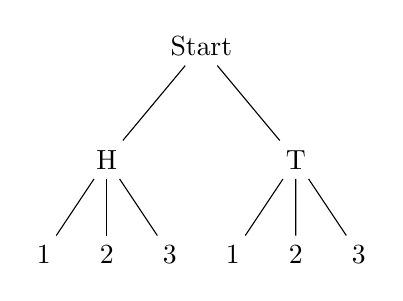
\begin{tikzpicture}[scale=0.8,
  level 1/.style={sibling distance=3cm, level distance=1.8cm},
  level 2/.style={sibling distance=1cm, level distance=1.5cm}]
  \node {Start}
    child {node {H}
      child {node {1}}
      child {node {2}}
      child {node {3}}
    }
    child {node {T}
      child {node {1}}
      child {node {2}}
      child {node {3}}
    };
\end{tikzpicture}
\end{center}
\end{questionText}
\choiceA{$3$}
\choiceB{$5$}
\choiceC{$6$}
\choiceD{$9$}
\correctAnswer{C}
\explanation{The tree shows $2$ branches (H, T) each splitting into $3$ sub-branches. Total: $2 \times 3 = 6$ outcomes.}
\end{practiceQuestion}

\begin{practiceQuestion}{9-5-q27}{gmc}
\begin{questionText}
The table below shows the sample space for rolling two dice. How many outcomes have a sum of $5$?

\begin{center}
\begin{tabular}{|c|c|c|c|c|c|c|}
\hline
 & \textbf{1} & \textbf{2} & \textbf{3} & \textbf{4} & \textbf{5} & \textbf{6} \\
\hline
\textbf{1} & $2$ & $3$ & $4$ & \cellcolor{funBlue!20}$5$ & $6$ & $7$ \\
\hline
\textbf{2} & $3$ & $4$ & \cellcolor{funBlue!20}$5$ & $6$ & $7$ & $8$ \\
\hline
\textbf{3} & $4$ & \cellcolor{funBlue!20}$5$ & $6$ & $7$ & $8$ & $9$ \\
\hline
\textbf{4} & \cellcolor{funBlue!20}$5$ & $6$ & $7$ & $8$ & $9$ & $10$ \\
\hline
\textbf{5} & $6$ & $7$ & $8$ & $9$ & $10$ & $11$ \\
\hline
\textbf{6} & $7$ & $8$ & $9$ & $10$ & $11$ & $12$ \\
\hline
\end{tabular}
\end{center}
\end{questionText}
\choiceA{$3$}
\choiceB{$4$}
\choiceC{$5$}
\choiceD{$6$}
\correctAnswer{B}
\explanation{Outcomes with sum $5$: $(1,4), (2,3), (3,2), (4,1)$ — that is $4$ outcomes (highlighted in the table).}
\end{practiceQuestion}

\begin{practiceQuestion}{9-5-q28}{gmc}
\begin{questionText}
The tree diagram shows the sample space for choosing a shirt color (Red, Blue) and a pant type (Jeans, Shorts, Khakis). Which of the following is a complete list of outcomes with a Blue shirt?

\begin{center}
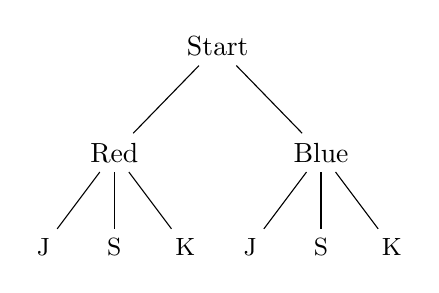
\begin{tikzpicture}[scale=0.75,
  level 1/.style={sibling distance=3.5cm, level distance=1.8cm},
  level 2/.style={sibling distance=1.2cm, level distance=1.6cm}]
  \node {Start}
    child {node {Red}
      child {node {\small J}}
      child {node {\small S}}
      child {node {\small K}}
    }
    child {node {Blue}
      child {node {\small J}}
      child {node {\small S}}
      child {node {\small K}}
    };
\end{tikzpicture}
\end{center}
\end{questionText}
\choiceA{Blue-Jeans, Blue-Shorts}
\choiceB{Blue-Jeans, Blue-Shorts, Blue-Khakis}
\choiceC{Red-Jeans, Red-Shorts, Red-Khakis}
\choiceD{Blue-Jeans only}
\correctAnswer{B}
\explanation{Following the Blue branch, there are $3$ sub-branches: Jeans, Shorts, Khakis. All three make up the Blue outcomes.}
\end{practiceQuestion}

\begin{practiceQuestion}{9-5-q29}{gsa}
\begin{questionText}
Use the table to find how many outcomes give a sum of $9$ when two dice are rolled. Write the number of outcomes.

\begin{center}
\begin{tabular}{|c|c|c|c|c|c|c|}
\hline
$+$ & \textbf{1} & \textbf{2} & \textbf{3} & \textbf{4} & \textbf{5} & \textbf{6} \\
\hline
\textbf{1} & $2$ & $3$ & $4$ & $5$ & $6$ & $7$ \\
\hline
\textbf{2} & $3$ & $4$ & $5$ & $6$ & $7$ & $8$ \\
\hline
\textbf{3} & $4$ & $5$ & $6$ & $7$ & $8$ & $9$ \\
\hline
\textbf{4} & $5$ & $6$ & $7$ & $8$ & $9$ & $10$ \\
\hline
\textbf{5} & $6$ & $7$ & $8$ & $9$ & $10$ & $11$ \\
\hline
\textbf{6} & $7$ & $8$ & $9$ & $10$ & $11$ & $12$ \\
\hline
\end{tabular}
\end{center}
\end{questionText}
\correctAnswer{$4$}
\explanation{Outcomes with sum $9$: $(3,6), (4,5), (5,4), (6,3)$ — that is $4$ outcomes.}
\end{practiceQuestion}

\begin{practiceQuestion}{9-5-q30}{gsa}
\begin{questionText}
The tree diagram shows the sample space for choosing a drink (Juice, Milk) and a snack (Apple, Banana, Cookie). List all outcomes and state the total number.

\begin{center}
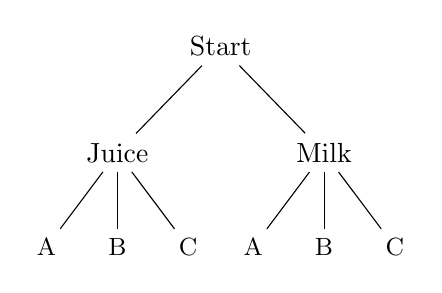
\begin{tikzpicture}[scale=0.75,
  level 1/.style={sibling distance=3.5cm, level distance=1.8cm},
  level 2/.style={sibling distance=1.2cm, level distance=1.6cm}]
  \node {Start}
    child {node {Juice}
      child {node {\small A}}
      child {node {\small B}}
      child {node {\small C}}
    }
    child {node {Milk}
      child {node {\small A}}
      child {node {\small B}}
      child {node {\small C}}
    };
\end{tikzpicture}
\end{center}
\end{questionText}
\correctAnswer{$6$ outcomes}
\explanation{Juice-Apple, Juice-Banana, Juice-Cookie, Milk-Apple, Milk-Banana, Milk-Cookie. Total $= 2 \times 3 = 6$.}
\end{practiceQuestion}
